\documentclass{article}

\usepackage[a4paper]{geometry}
\usepackage{graphicx}
\usepackage[utf8]{inputenc}
\usepackage{subcaption}
\usepackage{placeins}
\usepackage{wrapfig}
\usepackage{float}
\usepackage{minted}
\usepackage[noEnd=false]{algpseudocodex}
\usepackage{hyperref}

\graphicspath{{./images/}}

\newcommand{\code}[2]{\inputminted[linenos, breaklines, firstline=#1, lastline=#2]{c++}{Tema2.cpp}}

\title{Tema 2 --- Compresii de date}
\author{
    Mițca Dumitru\\
    Grupa NNNNL
}
\date{2023}

\begin{document}
    \maketitle

    \hypersetup{linkbordercolor=1 1 1}
    \renewcommand*\contentsname{Cuprins}
    \tableofcontents
    \hypersetup{linkbordercolor=1 0 0}

    \newpage

    \section{Prezentarea problemei}
    Compresia datelor devine din ce în ce mai necesară cu cât timpul trece.

    Numărul de utilizatori al internetului crește în fiecare an, la fel ca și cantitatea de date
    transmisă prin internet. Astfel dorința scăderii volumului transferat efectiv pe canalele
    internetului, cum reducerea numărului de utilizatori al internetului nu este
    fezabil\textsuperscript{[citation needed]}, compresia datelor devine soluția naturală.

    În această lucrare voi prezenta codificarea Huffman. Concepte similare de coficare sunt folosite în
    formate ca JPEG sau MP3 și in algoritmul Deflate (folosite de arhive de tipul gzip sau zip).

    \section{Prezentarea algoritmului}

    Algoritmul pentru compresarea unui șir folosind codificarea Huffman este următorul:

    \begin{algorithmic}[1]
        \State calculează frecvențele caracterelor din șir
        \State aplică algoritmul \texttt{lep} din Lucrarea 9 pe vectorul rezultat
        \State \texttt{rez} $\gets$ ""
        \ForAll{caracter $\in$ șir}
            \State obține codul Huffman a caracterului
            \State concatenează la finalul \texttt{rez} codul obținut
        \EndFor
        \State
        \Return \texttt{rez}
    \end{algorithmic}

    Algoritmul $lep$ este:
    \begin{algorithmic}[1]
        \Procedure{lep}{arguments}
            \State $B \gets \{t(x_0), \dots, t(x_{n-1})\}$
            \While $(\#B > 1)$
                \State alege $t_1, t_2$ din $B$ cu $info(rad(t_1)), info(rad(t_2))$ minime
                \State construiește arborele $t$ în care subarborii rădăcinii sunt $t_1, t_2$ și \\ \hphantom{lol} info(rad($t$)) = info(rad($t_1$)) + info(rad($t_2$))
                \State $B \gets (B \setminus \{t_1, t_2\}) \cup \{t\}$
            \EndWhile
        \EndProcedure
    \end{algorithmic}

    \section{Prezentarea programului}

    Programul începe cu include-urile necesare utilizării unor bibliotece:
    \code{1}{7}

    Apoi urmează definițiile structurile folosite în program:
    \code{9}{21}

    Programul folosește implementarea cu \emph{min-heap} pentru obținirea rădăcinilor de frecvență
    minimă din mulțimea \texttt{B}. Implementarea \emph{min-heap}-ului este următoare și se
    foloșeste de funcțiile \texttt{make\_heap}, \texttt{pop\_heap}, \texttt{push\_heap} din librăria
    standard C++:
    \code{23}{65}

    Pentru a putea aplica algoritmul de construire a unui arbore binar ponderat pe frontieră (necesar
    pentru construirea codurilor fără prefix asociate fiecărui caracter din șir), am folosit următorul
    algorithm:
    \code{67}{86}

    Construirea arborelui în sine folosește algoritmul prezentat în Laboratorul 9:
    \code{88}{106}

    Pentru a realiza conversia dintr-un șir de caractere într-un șir de biți, am scris
    un algoritm intermediar, care convertește un caracter într-un cod binar navigând
    arborele în mod recursiv.
    \code{108}{131}

    Pentru convertirea unui șir de caractere în versiunea codificată a sa, am folosit următoarea
    funcție, care pur și simplu iterează fiecare caracter din șir și îi obține reprezentarea binară.
    \footnote{O posibilă optimizare a acestei funcții ar fi stocarea reprezentării binare într-un
    tablou asociativ, asigurând astfel o singură iterare a arborelui pentru fiecare caracter. Această
    optimizare ar conduce la maxim 256 iterații ale arborelui, adică complexitatea funcției ar deveni
    $\mathcal{O}(n)$, în loc de $\mathcal{O}(n\cdot m)$, unde $n$ este lungimea șirului și $m$
    înălțimea arborelui.}
    \code{133}{143}

    Într-un final funcția \texttt{main} a programului citește un șir de caractere de la \texttt{stdin},
    îl compresează și apoi afișează statistici despre șirul compresat în relația cu șirul original:
    \code{145}{166}

    \newpage
    \section{Rulări}

    Rezultatele a câteva rulări sunt următoarele:
    \begin{figure}[H]
        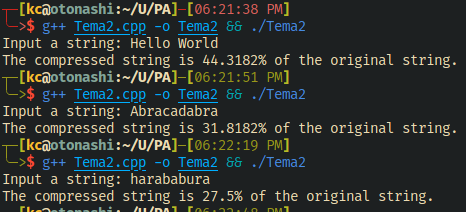
\includegraphics[width=0.75\linewidth]{Tema2Rulari}
        \centering
    \end{figure}
\end{document}
